
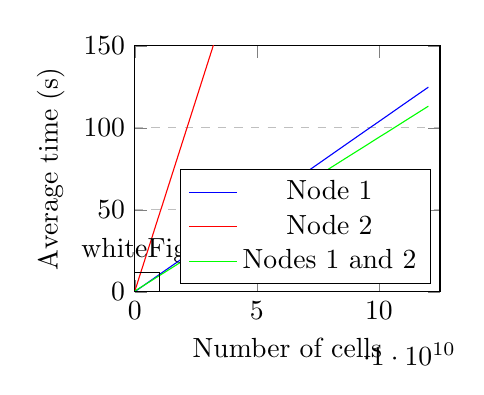
\begin{tikzpicture}
\begin{axis}[
    %title={Average time to compute edit distance},
    xlabel={Number of cells},
    ylabel={Average time (s)},
    xmin=0, xmax=125000000000,
    ymin=0, ymax=150,
    legend pos=south east,
    ymajorgrids=true,
    grid style=dashed,
    scaled x ticks={real:10000000000},
    width=0.45\linewidth,
]


\addplot[
    color=blue,
    smooth,
    ]
    coordinates {
    (16777216, 0.09921685714285713)(33554432, 0.12080128571428571)(67108864, 0.160687)(134217728, 0.2424785714285714)(268435456, 0.38340228571428575)(536870912, 0.6664877142857142)(1000000000, 1.152977142857143)(1500000000, 1.6785985714285712)(2147483648, 2.357917142857143)(3000000000, 3.2444357142857143)(4294967296, 4.582278571428572)(6000000000, 6.368568571428573)(7000000000, 7.4005728571428575)(8589934592, 9.062895000000001)(10000000000, 10.52197142857143)(11000000000, 11.564114285714284)(12000000000, 12.593114285714284)(13000000000, 13.643714285714285)(14000000000, 14.677214285714285)(17179869184, 17.97048571428571)(25769803776, 26.88624285714286)(34359738368, 35.8241)(42949672960, 44.70372857142858)(51539607552, 53.59438571428571)(60129542144, 62.536071428571425)(68719476736, 71.40738571428571)(77309411328, 80.32997142857143)(85899345920, 89.26152857142857)(94489280512, 98.17172857142855)(100000000000, 103.8337142857143)(103079215104, 107.02371428571429)(111669149696, 115.95128571428572)(120259084288, 124.80914285714286)
    };

\addplot[
    color=red,
    smooth,
    ]
    coordinates {
    (16777216, 0.5445155714285714)(33554432, 0.626533)(67108864, 0.8027252857142858)(134217728, 1.12474)(268435456, 1.7438942857142856)(536870912, 3.0209571428571427)(1000000000, 5.162437142857143)(1500000000, 7.543924285714286)(2147483648, 10.5999)(3000000000, 14.472014285714282)(4294967296, 20.55514285714286)(6000000000, 28.49077142857143)(7000000000, 33.10725714285714)(8589934592, 40.61537142857143)(10000000000, 47.16012857142857)(11000000000, 51.74827142857142)(12000000000, 56.35255714285715)(13000000000, 61.09289999999999)(14000000000, 65.73704285714287)(17179869184, 80.55284285714286)(25769803776, 120.55142857142857)(34359738368, 160.5607142857143)(42949672960, 200.45)(51539607552, 240.47842857142857)(60129542144, 280.283)(68719476736, 320.3165714285714)(77309411328, 360.40957142857144)(85899345920, 400.24628571428576)(94489280512, 440.2641428571429)(100000000000, 465.98900000000003)(103079215104, 480.2848571428571)(111669149696, 520.3457142857143)(120259084288, 560.304)
    };

\addplot[
    color=green,
    smooth,
    ]
    coordinates {
    (16777216, 0.496333)(33554432, 0.5080268571428571)(67108864, 0.6234567142857143)(134217728, 0.6975642857142856)(268435456, 0.7566615714285714)(536870912, 1.0175524285714288)(1000000000, 1.4202885714285713)(1500000000, 1.9164114285714287)(2147483648, 2.5176842857142856)(3000000000, 3.249014285714286)(4294967296, 4.516901428571428)(6000000000, 6.0832242857142855)(7000000000, 7.0254957142857135)(8589934592, 8.529228)(10000000000, 9.85383)(11000000000, 10.788914285714286)(12000000000, 11.679885714285714)(13000000000, 12.648942857142856)(14000000000, 13.559485714285714)(17179869184, 16.574385714285714)(25769803776, 24.604942857142856)(34359738368, 32.70814285714285)(42949672960, 40.747)(51539607552, 48.7744)(60129542144, 56.66547142857142)(68719476736, 64.66221428571428)(77309411328, 72.89688571428572)(85899345920, 81.01222857142857)(94489280512, 89.02959999999999)(100000000000, 94.25682857142858)(103079215104, 97.06402857142858)(111669149696, 105.15614285714285)(120259084288, 113.20742857142857)
    };

\addplot[
    color=black,
    mark=none,
] coordinates {(0,0) (0,12) (10000000000,12) (10000000000,0) (0,0)};

\pgfplotsset{
    after end axis/.code={
        \node[above] at (axis cs:10000000000,12){\contour{white}{Fig. \ref{result_graph_zoom}}};
    }
}


\legend{Node 1, Node 2, Nodes 1 and 2}
\end{axis}
\end{tikzpicture}
